% Set the document class and theme
\documentclass{beamer}
\usetheme{CambridgeUS}
\setbeamertemplate{caption}[numbered]
\setbeamertemplate{theorems}[numbered]
\setbeamerfont{footnote}{size=\tiny}

\usepackage{./presentation_macros}

\addbibresource{references.bib}

% Add presentation data here

% Text in the square brackets `[]' are shown in the footer. If not mentioned,
% then text in the curly braces `{}' are used as theme defaults.

\title[Zone Encryption]{Zone Encryption with Anonymous Authentication for V2V
Communication \\
\small Jan Camenisch, Manu Drijvers, Anja Lehmann, Gregory Neven and Patrick
Towa}
\date{April 23, 2024}
\author{Gautam Singh}
\institute[IITH]{Indian Institute of Technology Hyderabad}

% Presentation begins here

\begin{document}
    \maketitle
    \tableofcontents
    \section{Introduction}
    
    \begin{frame}
        \frametitle{V2X Related Terminology}
        \begin{figure}
            \centering
            \resizebox{.8\textwidth}{!}{\begin{tikzpicture}[
    mindmap,
    concept color=red!55!black,
    text=white
]
    \node [concept] {\textbf{V2X}\\\small{Vehicle-to-Everything}}
    child[grow=150] {node[concept] {\textbf{V2D}\\\tiny{Vehicle-to-Device}}}
    child[grow=210] {node[concept] {\textbf{V2G}\\\tiny{Vehicle-to-Grid}}}
    child[grow=0] {
        node[concept] {\textbf{V2N}\\\tiny{Vehicle-to-Network}}
        child[grow=60] {node[concept] {\textbf{V2C}\\\tiny{Vehicle-to-Cloud}}}
        child[grow=120] {node[concept] {\textbf{V2P}\\\tiny{Vehicle-to-Pedestrian}}}
        child[concept color=green,grow=240,text=black] {node[concept] {\textbf{V2V}\\\tiny{Vehicle-to-Vehicle}}}
        child[concept color=green,grow=300,text=black] {node[concept] {\textbf{V2I}\\\tiny{Vehicle-to-Infrastructure}}}
    };
\end{tikzpicture}}
            \caption{A breakdown of V2X.}
        \end{figure}
    \end{frame}

    \begin{frame}
        \frametitle{Message Types in V2X}
        \begin{enumerate}
            \item \textbf{Cooperative Awareness Messages} (CAMs)
            \footcite{etsi-en-302-637} and \textbf{Basic Safety Messages} (BSMs)
            \begin{enumerate}
                \item Exchanged between vehicles to create awareness and support
                cooperative performance of vehicles in the road network.
                \item Includes status information such as time, position, speed,
                active systems, vehicle dimensions, etc.
            \end{enumerate}
            \pause
            \item Other types of messages
            \begin{enumerate}
                \item \textbf{Signal Phase and Timing} (SPaT)
                \item \textbf{Roadside Infrastructure Information} (MAP)
            \end{enumerate} 
        \end{enumerate}
    \end{frame}

    \begin{frame}
        \frametitle{V2X and Cryptology}
        \begin{enumerate}
            \item CAMs broadcasted unencrypted in 5.9 GHz channel (ETSI ITS-G5).
            \begin{enumerate}
                \item Frequently broadcast: 1 CAM per second in US, 10 per
                second in EU.
                \item Easy to intercept.
                \item Leak sensitive information about the vehicle owners.
                \pause
                \item \textbf{Huge privacy concerns and threats!}
            \end{enumerate}
            \pause
            \item Encryption impractical, since CAMs \emph{must} be decrypted by
            nearby vehicles in a highly dynamic environment.
            \begin{enumerate}
                \item But CAMs \emph{have to} be encrypted because of the data
                they carry!
            \end{enumerate}
            \pause
            \item Instead, focus on \emph{privacy-preserving authentication}.
            \begin{enumerate}
                \item Ensuring a message is issued by a ``genuine'' vehicle.
                \item ``Genuine'' vehicles must be untraceable.
            \end{enumerate}
        \end{enumerate}
    \end{frame}

    \begin{frame}
        \frametitle{V2X and Cryptology}
        \begin{enumerate}
            \item Deployed systems
            \begin{enumerate}
                \item Use short-term \textbf{pseudonym certificates} (100 per
                week in EU, 20 per week in US), rotate between them.
                \item Trade-off between security (Sybil resistance), privacy and
                efficiency (storage and bandwidth costs).
            \end{enumerate}
            \pause
            \item Proposed systems
            \begin{enumerate}
                \item Stronger privacy and security guarantees.
                \item Do not meet the \emph{stringent bandwidth constraint} of
                \textbf{300 bytes per CAM}, thus impractical.
            \end{enumerate}
        \end{enumerate}
    \end{frame}

    \begin{frame}
        \frametitle{Motivation and Goals}
        \begin{enumerate}
            \item Unlimited privacy.
            \item Address problems of authenticity and confidentiality in
            combination \emph{for the first time}.
            \item Meet (bandwidth) requirements.
            \item Efficient encryption scheme (symmetric-key crypto).
            \item Negligible storage and bandwidth overheads.
            \item Better security guarantees (privacy, authenticity,
            confidentiality).
        \end{enumerate}
    \end{frame}

    \section{Preliminaries}

    \begin{frame}
        \frametitle{Preliminaries}
        \begin{enumerate}
            \item Pairing-based Cryptography
            \item Hardness Assumptions
            \begin{enumerate}
                \item Symmetric Discrete Logarithm (SDL) assumption
                \item Modified \(q\)-Strong Diffie-Hellman (q-MSDH-1) assumption
            \end{enumerate}
            \item Deterministic Authenticated Encryption (DAE)
            \item PS Signatures
            \item Dynamic Group Signatures with Attributes (DGS+A)
        \end{enumerate}
    \end{frame}

    \section{Zone Encryption}
    \begin{frame}
        \frametitle{Overall Flow of Zone Encryption}
        \begin{figure}[!ht]
            \centering
            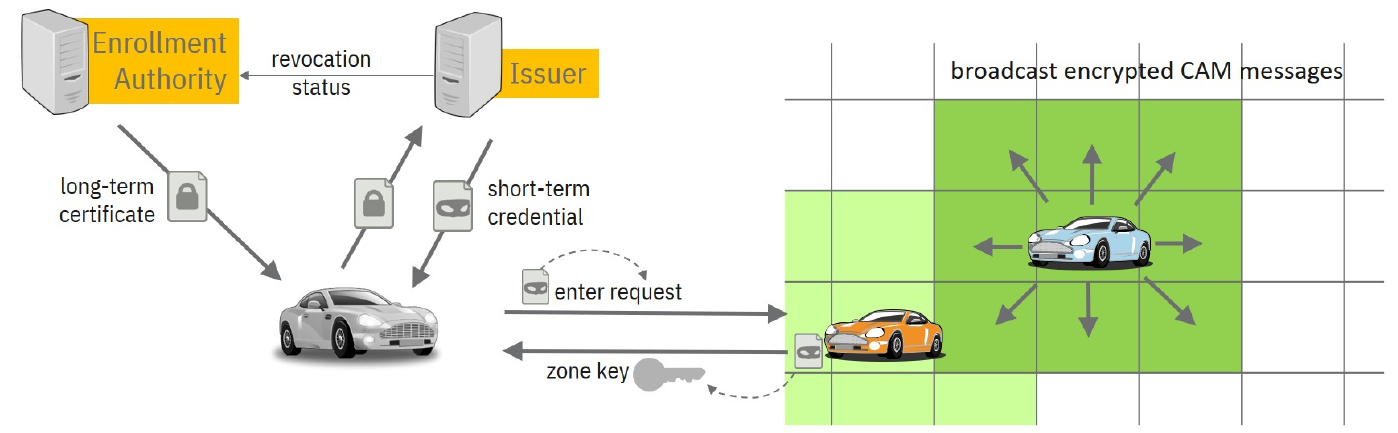
\includegraphics[width=\textwidth]{figs/ze_flow.png}
            \caption{Illustration of Zone Encryption with its Anonymous-Authentication Approach.}
        \end{figure}
    \end{frame}

    \begin{frame}
        \frametitle{Notation}
        \begin{table}[!ht]
            \centering
            \begin{tabular}{|c|c|}
                \hline
                \textbf{Notation} & \textbf{Meaning} \\
                \hline
                \(Z\) & Set of zones covering the road network \\
                \hline
                \(\cP\) & Payload/message space \\
                \hline
                \(Epoch\) & Set of epochs \\
                \hline
                \(T\) & Set of timestamps \\
                \hline
                \(K_{z,t}\) & Zone key for zone \(z\) at time \(t\) \\
                \hline
                \(L_K\) & List of zone keys known to a vehicle, stored as
                \(\brak{z,t,K_{z,t}}\) \\
                \hline
                \(\cE\) & Enrollment authority \\
                \hline
                \(\cI\) & Issuer \\
                \hline
                \(\cV \in \cbrak{0,1}^*\) & Vehicle identity \\
                \hline
                \(cert_{\cV}\) & Long-term certificate of \(\cV\) \\
                \hline
                \(cred_{\cV}\) & Short-term credential of \(\cV\) \\
                \hline
            \end{tabular}
        \end{table}
    \end{frame}

    \begin{frame}
        \frametitle{Zones, Epochs, Zone Keys}
        \begin{columns}
            \begin{column}{0.7\textwidth}
                \begin{enumerate}
                    \item A \emph{zone} \(z\) is a continuous geographical area
                    covering part of a road network (shown as squares alongside).
                    \item<2-> Each zone has a \emph{zone key} \(K_{z,t}\) periodically
                    refreshed after a time interval called an \emph{epoch}.
                    \begin{itemize}
                        \item An epoch is denoted by \(\rbrak{\lsbrak{e,e+1}}\).
                        Each time instance \(t\) satisfies \(e \le t < e + 1\)
                        for a unique \(e\). This is denoted as \(e\brak{t}\).
                        \item Vehicles need \(K_{z,t}\) for secure communication
                        when they are in zone \(z\) at time \(t\).
                    \end{itemize}
                    \item<3-> Vechicles can communicate securely with other
                    vehicles in surrounding zones also.
                \end{enumerate}
            \end{column}
            \begin{column}<1->{0.3\textwidth}
                \begin{figure}
                    \centering
                    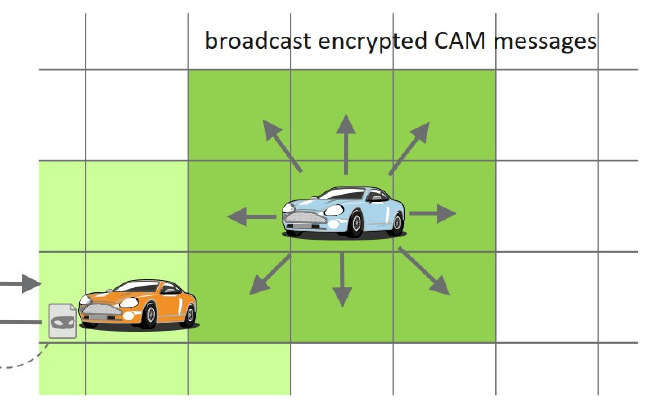
\includegraphics[width=\columnwidth]{figs/ze_zones.png}
                    \caption{A vehicle must have the zone keys of zones adjacent to it. It can communicate with another vehicle if they share a zone key.}
                \end{figure}
            \end{column}
        \end{columns}
    \end{frame}

    \begin{frame}
        \frametitle{Entities and Credentials}
        \begin{columns}
            \begin{column}{0.7\textwidth}
                \begin{enumerate}
                    \item An \emph{enrollment authority} \(\cE\) issues
                    \emph{long-term certificates} to vehicle \(\cV \in
                    \cbrak{0,1}^*\).
                    \begin{enumerate}
                        \item Long-term certificate \(cert_{\cV}\)
                        obtained.
                        \item Can be used to check revocation status.
                    \end{enumerate}
                    \item<2-> An \emph{issuer} \(\cI\) issues
                    \emph{short-term credentials} to vehicles every epoch.
                    \begin{enumerate}
                        \item Long-term credential \(cert_{\cV}\) used
                        here.
                        \item Short-term credential \(cred_{\cV}\)
                        obtained.
                        \item \(cred_{\cV}\) is valid only for the epoch
                        \(e\) in which it was issued.
                    \end{enumerate}
                \end{enumerate}
            \end{column}
            \begin{column}<1->{0.3\textwidth}
                \begin{figure}
                    \centering
                    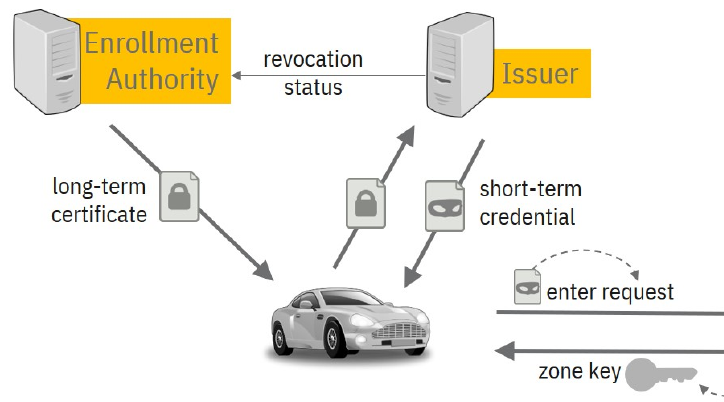
\includegraphics[width=\columnwidth]{figs/ze_entities.png}
                    \caption{Various entities and exchanged credentials in ZE.}
                \end{figure}
            \end{column}
        \end{columns}
    \end{frame}

    \begin{frame}
        \frametitle{Syntax of ZE}
        \begin{block}{Setup and Key Generation}
            \begin{enumerate}
                \item \(\mathsf{Setup}\brak{1^{\lambda},Z,Epoch,T} \rightarrow
                pp\)
                \item \(\mathsf{KG.E}\brak{pp} \rightarrow
                \brak{pk_{\cE},\brak{sk_{\cE},\red{st_{\cE}}}}\)
                \begin{itemize}
                    \item State keeps track of enrolled vehicles.
                \end{itemize}
                \item \(\mathsf{KG.I}\brak{pp} \rightarrow
                \brak{pk_{\cI},\brak{sk_{\cI},\red{st_{\cI}}}}\)
                \begin{itemize}
                    \item State keeps track of open messages sent during key
                    requests.
                \end{itemize}
            \end{enumerate}
        \end{block}
        \pause
        \begin{block}{Receiving Long-term and Short-term Credentials}
            \begin{enumerate}
                \item \(\abrak{\mathsf{Enroll.V}\brak{pk_{\cE},\cV}
                \leftrightharpoons
                \mathsf{Enroll.E}\brak{sk_{\cE},st_{\cE},\cV}} \rightarrow
                \abrak{cert_{\cV},st_{\cE}^{\prime}}\)
                \item
                \(\abrak{\mathsf{Authorize.V}\brak{\red{cert_{\cV}},e,pk_{\cI}}
                \leftrightharpoons
                \mathsf{Authorize.I}\brak{sk_{\cI},st_{\cI},\cV,e,\red{pk_{\cE}}}}
                \rightarrow \abrak{cred_{\cV},st_{\cI}^{\prime}}\)
                \begin{itemize}
                    \item Vehicle uses certificate to obtain credentials.
                    \item Issuer checks certificate using public key of issuer.
                \end{itemize}
            \end{enumerate}
        \end{block}
    \end{frame}

    \begin{frame}
        \frametitle{Syntax of ZE}
        \begin{block}{Entering and Exiting Zones}
            \begin{enumerate}
                \item \(\langle
                \mathsf{Enter.V}\brak{cred_{\cV},L_K,pk_{\cI},z,t,requester}
                \leftrightharpoons
                \mathsf{Enter.W}\brak{cred_{\cW_i},L_{K_i},pk_{\cI},z,t,responder_i}_{i\ge
                0} \rangle \rightarrow \abrak{L_K,\perp}\)
                \begin{itemize}
                    \item Why \(i \ge 0\)?
                \end{itemize}
                \item \(\mathsf{Exit}\brak{L_K,z,t} \rightarrow L_K^{\prime}\)
            \end{enumerate}
        \end{block}
        \begin{block}{Sending and Receiving Payloads}
            \begin{enumerate}
                \item \(\mathsf{Send}\brak{L_K,P,\red{Y\subseteq Z},t}
                \rightarrow \gamma/\perp\)
                \item \(\mathsf{Receive}\brak{L_K,\gamma} \rightarrow P/\perp\)
                \item It's all symmteric key cryptography! (But what is the
                symmetric key?)
            \end{enumerate}
        \end{block}
    \end{frame}

    \begin{frame}
        \frametitle{Syntax of ZE}
        \begin{block}{Identity Escrow}
            \begin{enumerate}
                \item \(\mathsf{Open}\brak{sk_{\cI},st_{\cI},\red{m}}
                \rightarrow \cV/\perp\)
                \item \(m\) is a message that was sent during an execution of
                \textsf{Enter}.
                \item Only \(\cI\) can find which vehicle sent \(m\).
                \item Use cases
                \begin{itemize}
                    \item To revoke certificates of misbehaving vehicles.
                    \item To provide concrete court evidence.
                \end{itemize}
                \item Assuming identity escrow is rare, \textsf{Open} need not
                be efficient in terms of time/storage complexity.
            \end{enumerate}
        \end{block}
    \end{frame}

    \begin{frame}
        \frametitle{Security of ZE}
        \begin{enumerate}
            \item \textbf{}
        \end{enumerate}
    \end{frame}

    \begin{frame}
        \frametitle{Instantiation of ZE and Efficiency}    
        (Is it worth mentioning section 4.4.1 or can we leave this?)
    \end{frame}

    \begin{frame}
        \frametitle{Summary of ZE}
        Table 2 of the paper.
    \end{frame}

    \section{Group Signatures with Attributes}
    \begin{frame}
        \frametitle{DGS+A}
        Sub-headings
        \begin{enumerate}
            \item Syntax
            \item Security properties (no proofs)
            \item Instantiation from PS
            \item Can be extended to threshold opening (should be a slide or
            only a mention during talk?)
        \end{enumerate}
    \end{frame}

    \section{Conclusion}
    \begin{frame}
        \frametitle{Challenges in Deploying ZE}
        Section 4.6
    \end{frame}

    \begin{frame}
        \frametitle{Future Improvements}
        Section 4.6, brief and top-level idea of mini-project if time permits.
    \end{frame}
\end{document}
